\documentclass[11pt,a4paper]{article}
\usepackage[utf8]{inputenc}
\usepackage[T1]{fontenc}
\usepackage{lmodern}
\usepackage[margin=2.5cm]{geometry}
\usepackage{graphicx}
\usepackage{microtype}
\usepackage{csquotes}
\usepackage[hidelinks]{hyperref}
\setlength{\parskip}{0.5em}
\setlength{\parindent}{0pt}

%% Generated from paper.md by scripts/paper_md_to_tex.py - do not edit by hand.
%% Edit paper.md and regenerate, so the two versions cannot diverge.

\title{Before the Backtest: Pre-Freeze Common-Support Ceilings for Event-Driven Strategy Research}
\date{2026-10-11}
\author{}
\begin{document}
\maketitle


\textbf{Working paper, V3.} 2026-10-11. Single-contribution restructure after referee report V2.


\begin{quote}
\textbf{Relationship to V1 and V2.} V1 (\texttt{paper.md}, SHA-256 \texttt{1853bce0\ldots{}}) and V2 (\texttt{paper\_v2.md}, SHA-256 \texttt{b2c3ddae\ldots{}}) are frozen and are not edited. V3 is a restructure around one contribution, not a patch on V2. Every V2$\rightarrow$V3 change is listed in \texttt{PAPER\_V3\_FREEZE.md}. No experiment was run, no verdict changed, and no number produced by an experiment was recomputed.
\end{quote}



\section*{Abstract}


Matched event studies require that, for each event, a comparable control set exists. In event-driven strategy research this requirement interacts with two constraints that are absent from most applied settings: entity eligibility changes over time, so the control universe must be reconstructed point-in-time, and the outcome --- a price --- is always already available to the researcher, so nothing prevents the design from being adjusted after it is seen.


The design-stage principle is established: Rubin (2008) argues that observational studies must be designed without examining outcome data, and that a candidate dataset may have to be rejected for lack of covariate overlap. Overlap is normally diagnosed on the assembled analysis sample. We describe and apply a narrower variant: a \textbf{pre-freeze common-support ceiling}, in which the maximum attainable matched support is computed at each event time on the \textbf{complete point-in-time eligible population}, before the design is frozen and before any outcome column is opened, and compared against a pre-registered minimum. If the implied confirmatory sample falls below the minimum, the study is \texttt{DESIGN INFEASIBLE UNDER THIS SPECIFICATION} and does not proceed.


We demonstrate it on 62 candidate cryptocurrency delisting events with an exact matching rule on liquidity band and public-warning state and a floor of 20 matched controls. The realised distribution of matched controls per event is p10 0, p25 0, median 1, p75 2, p90 57, with 52 of 62 events below the floor. Computed on the complete eligible pool with no sampling, the per-date ceiling ranges from 0 to 27 warned assets with a median of 7, and only 3 of 25 announcement dates reach 20. The implied confirmatory sample is 10 against a pre-registered minimum of 40, so the study stopped before freeze. No price column was ever loaded: the data loader requested four non-price fields, which makes the outcome-blindness of the decision checkable from source. Supporting material establishes that the event population and the control universe can be reconstructed point-in-time at all.


\textbf{Keywords:} common support, positivity, outcome-free design, point-in-time data, event studies, pre-registration, research feasibility.



\section*{1. Introduction}


\subsection*{1.1 The question}


Matched and controlled event designs rest on a condition that is easy to state and easy to assume: for each treated event, the data must contain comparable untreated units. When that condition fails, no estimator recovers the intended comparison; it either fails to run, or runs on an implicitly redefined population.


This paper asks a narrow question:


\begin{quote}
\textbf{Can an event-study design be shown to lack adequate common support before any outcome is opened?}
\end{quote}


The answer we report is yes, for a particular class of designs, by a particular procedure, and at a measurable cost.


\subsection*{1.2 What is already established}


The principle that design precedes analysis is not new, and this paper does not claim it. Rubin (2008) argues that observational studies must be designed \textbf{without examining any outcome data}, and states explicitly that a candidate dataset may have to be rejected as inadequate for lack of covariate data or lack of overlap between treated and control groups, revealed by propensity-score analysis. That is the design-stage rejection this paper operationalises, and it is Rubin's.


Three further literatures bound what follows. Positivity --- the requirement that every covariate stratum occurring among the treated also occurs among controls --- is formalised in causal inference, with diagnostics and remedies including restricting the adjustment set, restricting the sample, or modifying the target intervention (Petersen et al. 2012). Overlap diagnostics are implemented as design-stage tools that are explicitly run before outcome data are used, for example in the design module of the \texttt{PSweight} package, which visualises overlap and assesses balance prior to outcome analysis; and the outcome-free two-stage design has been codified for regulatory submissions (Li 2023). Separately, the systematic-strategy literature establishes that reported performance must be discounted for the number of specifications tried (Bailey \& López de Prado 2014), that published anomalies replicate poorly (Hou, Xue \& Zhang 2020), and that analyst discretion alone produces substantial dispersion on identical data (Menkveld et al. 2024).


\subsection*{1.3 The gap, stated cautiously}


Overlap is normally diagnosed \textbf{on the assembled analysis sample}: the researcher builds the study, then inspects whether the treated and control distributions overlap. Two features of event-driven strategy research make that ordering insufficient.


First, \textbf{eligibility is time-varying}. Entities list, delist, change instrument coverage and change regulatory state. The set of admissible controls at one event date is not the set at another, and neither is the set available today. An overlap diagnostic run on whatever sample was assembled cannot distinguish "the sample is small" from "the population could never have supplied a sample".


Second, \textbf{the outcome is always already available}. In a clinical or regulatory setting, outcome blinding is partly enforced by data arriving later. In strategy research the price history sits in the same archive as everything else, so blinding is procedural, and procedural blinding is exactly what a reader cannot verify.


We therefore describe a variant with three specific properties: the support is computed on the \textbf{complete point-in-time eligible population} rather than on an assembled sample; the result is compared against a \textbf{pre-registered numeric minimum} that converts the diagnosis into a binding stop rule rather than a judgement; and outcome-blindness is enforced \textbf{structurally}, at the data-access layer, so it can be audited from source.


\begin{quote}
\textbf{Novelty, bounded.} We are not aware of prior work that operationalises common-support feasibility in this exact pre-freeze, full-population, outcome-blind form, with a pre-registered numeric stop rule, for matched event studies in systematic strategy research. We do \textbf{not} claim that common support, positivity diagnostics, matching feasibility, outcome-free design or design-stage rejection are new. Each is established, and Rubin (2008) states the design-stage rejection directly.
\end{quote}


\subsection*{1.4 Domain}


The claims in this paper apply to: event-driven systematic research; event populations assembled from public institutional documents and venue archives; free or public historical data; matched or otherwise controlled event designs; and settings in which entity lifecycle and eligibility change over time.


They are \textbf{not} claims about all quantitative research, all asset classes, all institutional desks, or all systematic strategies. \S{}7 reports the research registry that bounds them.


\subsection*{1.5 Contribution and roadmap}


This paper makes one methodological contribution and reports one empirical demonstration of it.


The \textbf{contribution} is the pre-freeze common-support ceiling of \S{}2: a procedure that takes a proposed event set, a point-in-time control universe, an intended matching rule and a pre-registered minimum, and returns a design-feasibility verdict before the outcome is opened. Its status as a contribution rests on the combination set out in \S{}2.6, not on any component.


The \textbf{demonstration} is \S{}4: a design that looked well-resourced at 62 events with near-complete data, and that the audit showed could never have been estimated under its own specification. The verdict was reached with no price column loaded, which \S{}2.5 makes checkable.


Everything else is support. \S{}3 establishes that the inputs exist. \S{}5 sets out what the gate prevents and, equally, what it does not justify. \S{}6 reports three results that bound the demonstration: that the population is reconstructible at all, that point-in-time validity must extend to classification logic, and that passing a feasibility gate does not substitute for out-of-sample falsification. \S{}7 reports the full research registry, which shows that this paper's cases were selected after the fact and does not support a broader thesis. \S{}8 states the limitations, which are substantial.


\subsection*{1.6 Two definitions}


\textbf{Point-in-time (PIT).} A quantity is point-in-time with respect to a decision at time \emph{t} if it is constructible from records whose publication or observation time precedes \emph{t}. A value that is numerically correct and correctly dated can still fail this test if the rule that assigned it used information published after \emph{t} (Supporting Case B).


\textbf{Common support.} Two groups have common support over a covariate set if every covariate stratum occurring among the treated also contains comparison units. Under an exact matching rule it is a counting condition: the matched cell must be non-empty at the required size. This is the finite-sample form of positivity.



\section*{2. The design principle: pre-freeze feasibility}


\subsection*{2.1 Point-in-time eligible universe}


Let \emph{E} be the proposed event set and \emph{t\_e} the time of event \emph{e}. The candidate control universe \texttt{C(t\_e)} is constructed from information available by \emph{t\_e} only. Two rules do the work.


A current instrument or entity list may not be used as history. An entity that exists now need not have existed at \emph{t\_e}, and an entity that existed then may have been removed since; in our setting both directions occur. And an identifier is not an identity: where symbols can be reassigned, the key is (entity, era), so a control is admitted only if the symbol belonged to the same entity at \emph{t\_e}.


Eligibility is evaluated as of \emph{t\_e} and never afterwards. In particular, a control that is removed \textbf{after} \emph{t\_e} remains a valid control at \emph{t\_e}; excluding it would use the future.


\subsection*{2.2 The proposed matching design}


The matching rule \texttt{M(e, c, t)} is written in full before the ceiling is computed, including the exact strata. In the demonstration it is exact matching on a liquidity band and on the entity's public-warning state at \emph{t\_e}, with a minimum of \emph{m} matched controls per event and a minimum admissible confirmatory sample of \emph{N\_min} events.


The rule is the object under test. A different rule is a different design, with a different ceiling, and the audit says nothing about it.


\subsection*{2.3 The full-pool support ceiling}


\begin{quote}
\textbf{PROCEDURE --- PRE-FREEZE COMMON-SUPPORT AUDIT} \textbf{Input:} event set \emph{E}; complete PIT candidate-control universe \texttt{C(t)}; matching function \texttt{M(e, c, t)}; minimum controls per event \emph{m}; minimum admissible event count \emph{N\_min}. For each event \emph{e} at time \emph{t\_e}: 1. construct \texttt{C(t\_e)} from information available by \emph{t\_e}; 2. exclude controls ineligible under the PIT rules of \S{}2.1; 3. apply the exact proposed matching rule; 4. compute the attainable support \textbf{S\_e = |\{ c ∈ C(t\_e) : M(e, c, t\_e) = 1 \}|}; 5. form the support indicator \textbf{I\_e = 1[S\_e $\geq$ m]}; 6. form the maximum confirmatory sample implied by the design \textbf{N\textbackslash{}\emph{ = Σ\_e I\_e}. \textbf{Decision.} If \textbf{N\textbackslash{}} < N\_min}, stop before outcome access. \textbf{Status:} \texttt{DESIGN INFEASIBLE UNDER THIS SPECIFICATION}.
\end{quote}


Two properties distinguish \texttt{S\_e} from a conventional overlap diagnostic.


\textbf{It is an upper bound, not an observation.} \texttt{S\_e} is computed over the complete eligible pool \texttt{C(t\_e)}, so any realised matched set is a subset of the set it counts. If the researcher evaluates only \emph{k} candidates per event date, as is normal when each candidate requires a data fetch, the realised count is at most \texttt{S\_e} and typically below it. This matters for the decision the audit supports: a low realised count is ambiguous between "we did not look hard enough" and "there is nothing to find", and a low \textbf{ceiling} is not. When the ceiling is below the floor, no additional sampling effort, no larger candidate draw and no further data collection can change the verdict, and the researcher is spared the cycle of enlarging the search in the hope that the cell fills.


\textbf{It is per-event, not pooled.} A pooled overlap statistic averages over event dates and can be dominated by a minority of well-supported events. In our demonstration the realised distribution is bimodal, with a p90 of 57 and a median of 1: pooled, the design looks partially supported; per event, most events have no comparison set at all. The quantity the design actually needs is the count of events clearing the floor, which is why the audit aggregates to \texttt{N*} by counting indicators rather than by averaging support.


\textbf{What the audit does not do.} It does not evaluate whether the matching covariates are the right ones, whether unobserved confounding remains after matching, or whether the estimand is interesting. It answers one question --- can the specified comparison be formed --- and a design that passes it can still be badly identified for every other reason.


\subsection*{2.4 The freeze and stop rule}


The audit is run \textbf{before} the pre-registration is frozen. This ordering is the point. If the ceiling is computed after the freeze, a researcher facing an empty cell must either abandon a registered design or amend it, and the amendment is made with knowledge of the scarcity. If it is computed before, the design that gets frozen is one that could have been estimated, and the design that cannot be is recorded as infeasible without ever having been registered.


\emph{m} and \emph{N\_min} must be fixed before the audit, for the same reason: a floor chosen after seeing the distribution of \texttt{S\_e} is not a floor.


\textbf{The status is a statement about the design, not about the world.} \texttt{DESIGN INFEASIBLE UNDER THIS SPECIFICATION} is not a null result, not a rejected hypothesis, and not evidence that the effect of interest is absent. The hypothesis is untested. This distinction is not a technicality: a research record that files infeasible designs as nulls will accumulate a literature of absences that were never measured.


\subsection*{2.5 Structural outcome blinding}


The credibility of the stop depends on knowing that no outcome informed it. Procedural blinding --- the researcher states that outcomes were not examined --- cannot be checked by a reader.


We therefore enforce blinding at the data-access layer. The feasibility loader requests four fields: open time, base volume, quote volume and trade count (\texttt{usecols=[0, 5, 7, 8]}). The OHLC columns never enter memory. No return, VWAP, basis, funding direction or derivative-relative move can be computed from what was read, by intent or by accident, and a reader can verify this by reading twenty lines of the loader rather than by trusting a sentence.


When a design fails this audit, the failure is therefore an \textbf{outcome-blind design failure}: it is known that no outcome could have influenced the decision, because no outcome was accessible to the process that made it.


\subsection*{2.6 What this inherits, and what it adds}


The components are not new and it is worth being exact about which part is which.


\textbf{Inherited: the design stage itself.} Rubin (2008) states the principle and the consequence directly --- observational studies are to be designed without examining outcome data, and a candidate dataset may have to be rejected as inadequate for lack of overlap between treated and control groups. A reader who takes only that from this paper has taken the main idea, and it is Rubin's. The same applies to the outcome-free two-stage design as it has been codified for regulatory submissions (Li 2023), and to design-stage overlap diagnostics implemented as tooling that runs before outcome data are used.


\textbf{Inherited: the statistical object.} Common support is the finite-sample face of positivity, whose diagnosis and remedies --- restricting the adjustment set, restricting the sample, modifying the target intervention --- are established, as is the distinction between violations that are structural and those that are artefacts of a finite sample (Petersen et al. 2012). Our \S{}4 result is read against that distinction rather than discovering it.


\textbf{Added, narrowly, and only in combination.} Three features of the variant described in \S{}2.1--\S{}2.5 are not, as far as we are aware, combined in prior work for this class of study.


\begin{enumerate}
\item \textbf{The support is computed on the complete point-in-time eligible population}, reconstructed
\end{enumerate}
   separately at each event time, rather than on the sample the researcher has assembled. In settings    with time-varying eligibility this is a different quantity: it separates "our sample is small"    from "the population could not have supplied a sample", and only the second licenses a stop.

\begin{enumerate}
\item \textbf{The result is compared against a numeric minimum fixed before the audit}, which converts a
\end{enumerate}
   diagnostic into a binding rule. Rubin's formulation --- a dataset \emph{may have to be} rejected --- leaves    the judgement with the analyst. Fixing \emph{m} and \emph{N\_min} in advance removes the discretion at the    moment it would otherwise be exercised, which is the moment the researcher discovers the cell is    empty.

\begin{enumerate}
\item \textbf{Outcome-blindness is enforced structurally rather than procedurally}, at the data-access layer
\end{enumerate}
   (\S{}2.5). In settings where outcome data arrive later, blinding is partly enforced by time. In    strategy research the price is in the same archive as the covariates, so the only verifiable    blinding is one a reader can check in the code.


We state this as an absence of awareness rather than as priority. If the combination has been formalised elsewhere, the contribution of this paper reduces to the empirical demonstration in \S{}4, which stands on its own.



\section*{3. Research setting and data construction}


The demonstration requires four things to exist before the audit is meaningful: a validated event population, a point-in-time instrument history, a point-in-time identity rule, and the matching covariates. This section establishes them and nothing else; the construction work that produced them is summarised in \S{}6 and detailed in Appendix A.


\textbf{Setting.} Full-asset delistings announced by a single cryptocurrency venue, 2018-10-12 to 2026-09-24, with the corresponding perpetual futures contracts. The venue publishes both its delisting notices and a historical archive of market data for instruments it has removed, which is what makes a point-in-time reconstruction possible at all (\S{}6.1).


\textbf{Event population.} 201 validated asset-level full-delisting events. The validation is described in \S{}6.1; recall against an independent, market-data-derived definition of cessation is 0.9801.


\textbf{Instrument history.} Terminated and current derivative contracts are equally observable in the archive (1.0 and 1.0), with missingness differentials of 0.0 pp by year, liquidity bucket, timestamp precision and notice order, so the PIT control universe of \S{}2.1 can be built without a coverage asymmetry between surviving and removed instruments.


\textbf{Identity.} Keys are (asset, era). An identity guard rejected one candidate mapping in which an archive symbol belonged to an asset that had acquired the ticker four years after the event.


\textbf{Matching covariates.} The liquidity band is computed from the entity's own pre-event traded notional. The public-warning state is the venue's published risk tag: 134 assets have ever carried it, across 28 notices, and the tag universe was verified against six notice vocabularies.


\textbf{Why this setting is a fair test of the procedure, and where it is favourable.} It is favourable in one respect: the venue publishes both its decisions and its historical market data, including for instruments it has removed, so the point-in-time population of \S{}2.1 is constructible at all. In most settings it would not be, and the audit would be impossible rather than informative --- which is itself a finding about where the procedure can be applied (\S{}6.1).


It is unfavourable, and therefore a fair test, in three respects. The event count is small by the standards of equity event studies, so an infeasibility verdict is not surprising and the procedure earns little credit for reaching it. The matching covariate that binds --- the public warning --- is a rare state by construction, since a venue that warned most of its listings would not be warning anyone. And the researcher had every incentive to find the design feasible: the question had no prior empirical answer, the data quality was unusually good, and the alternative to proceeding was a null result with nothing to report. The audit returned infeasible anyway, before any of that could be weighed against an observed outcome.



\section*{4. Empirical demonstration}


\subsection*{4.1 From event population to candidate design}


\begin{center}
\footnotesize
\begin{tabular}{p{0.307\linewidth}p{0.307\linewidth}p{0.307\linewidth}}
\hline
\textbf{step} & \textbf{events} & \textbf{basis} \\
\hline
validated full-delisting events & \textbf{201} & \S{}3 \\
Tier-1 USD\textcircled{\scriptsize S}-M perpetual live at \emph{t\_e} & \textbf{75} & instrument existence at the event, not today \\
materially shortable at \emph{t\_e} & \textbf{64} & minutes with actual trading after \emph{t\_e}, not merely a served candle \\
clean public-information events & \textbf{63} & no prior derivative notice \\
candidates for the matched design & \textbf{62} & one asset's derivative is coin-margined, so a USD\textcircled{\scriptsize S}-M design returns nothing for it \\
\hline
\end{tabular}
\end{center}


Sixty-two events, with near-complete data: spot 1-minute coverage 100\%, perpetual 98.41\%, synchronised minutes in the primary window 98.41\% with a median of 100\%, and 62 of 63 events clearing a pre-specified usability bar of 50. \textbf{By every data-quality measure the design looked well-resourced.}


\subsection*{4.2 The intended matching rule}


Each event is matched to controls in the same liquidity band \textbf{and} the same public-warning state at \emph{t\_e}, requiring \emph{m} = 20 matched controls per event, at least 73 valid 15-minute both-legs-traded transitions per event, and \emph{N\_min} = 40 confirmatory events.


The warning-state stratum is not decorative, and the design does not survive dropping it. The question is whether the derivative market moves ahead of the spot announcement in a way the spot market does not. \textbf{52 of the 62 event assets carried the venue's public risk warning before the announcement.} A comparison that does not hold the warning state fixed therefore contrasts publicly-warned, visibly deteriorating assets against generic healthy ones, and any divergence it measures is at least as plausibly the market's response to the public warning --- information everyone had --- as it is an anticipation of the announcement. The stratum is what separates the hypothesis from its leading rival.


The liquidity band plays a smaller but still necessary role: these are among the least liquid instruments on the venue, and spot and derivative legs of illiquid pairs diverge mechanically when arbitrage capacity is limited, independently of any information. Matching on liquidity does not remove that channel, but it stops it from being confounded with the treatment.


\subsection*{4.3 The central result: realised support and the full-pool ceiling}


\textbf{Realised support.} The distribution of matched controls per event is bimodal:


\begin{center}
\footnotesize
\begin{tabular}{p{0.184\linewidth}p{0.184\linewidth}p{0.184\linewidth}p{0.184\linewidth}p{0.184\linewidth}}
\hline
\textbf{p10} & \textbf{p25} & \textbf{median} & \textbf{p75} & \textbf{p90} \\
\hline
0 & 0 & \textbf{1} & 2 & 57 \\
\hline
\end{tabular}
\end{center}


\textbf{52 of 62 events} fall below the floor of 20. Events whose asset was not warned find large pools; events whose asset was warned find almost none --- and 52 of the 62 event assets were warned.


\textbf{The ceiling.} Computed on the \textbf{complete} eligible pool with no sampling, the number of assets simultaneously warned, still listed, not yet delisted, and carrying both a live perpetual and a live spot route ranges from \textbf{0 to 27} across announcement dates, with a \textbf{median of 7}. Only \textbf{3 of 25 dates reach 20} --- and that is before the liquidity band is matched at all.


The arithmetic behind the ceiling is simple and is the reason the result is structural rather than a sampling artefact: the venue has warned \textbf{134 assets in total, ever}. At any given announcement date, the subset simultaneously still listed, not yet delisted and carrying both instruments is roughly seven. Requiring twenty of them, in the event's own liquidity band, cannot be satisfied by collecting more data. Raising the per-date evaluation from 120 candidates to the full pool would move the median matched cell from 1 to roughly 3, not to 20.


\textbf{Two checks confirm the constraint is the matching cell and not the pipeline.} Availability is not binding: 2,857 of 2,877 evaluated non-event legs (99.3\%) clear the availability bar. And the transition filter never binds: zero events had at least 20 candidates of which fewer than 20 survived it. The cell is empty before any downstream filter is reached.


\subsection*{4.4 The stop}


Applying \S{}2.3 with \emph{m} = 20 and \emph{N\_min} = 40:


\begin{center}
\footnotesize
\begin{tabular}{p{0.460\linewidth}p{0.460\linewidth}}
\hline
\textbf{quantity} & \textbf{value} \\
\hline
candidate events & 62 \\
events meeting the support requirement, \textbf{N\textbackslash{}}* & \textbf{10} \\
required minimum, \emph{N\_min} & \textbf{40} \\
implied development / holdout split & 9 / 1 \\
\hline
\end{tabular}
\end{center}


A one-event holdout is not a holdout. \textbf{N\textbackslash{}* = 10 < 40}, so the study stopped.


\textbf{The stop does not depend on the choice of floor.} The floor \emph{m} = 20 is an engineering judgement (\S{}8), which invites the obvious objection that a lower floor would have rescued the design. It would not, and this can be read off the already-reported quantiles without recomputing anything. The 75th percentile of attainable support is \textbf{2}, so at most 25\% of the 62 events --- at most \textbf{15} events --- have more than two matched controls. Therefore for \textbf{any floor m $\geq$ 3}, the implied confirmatory sample satisfies \textbf{N\textbackslash{}\emph{ $\leq$ 15}, against }N\_min\emph{ = 40. The 90th percentile is 57, so at most six events have more than 57 controls, and N\textbackslash{}} falls to roughly 6 at the top of the range.


In other words, the verdict is invariant across the entire range of floors from 3 upward: no defensible choice of \emph{m} produces a confirmatory sample of 40. The design fails not because the bar was set high but because the distribution of attainable support is concentrated at zero and one. The bound is arithmetic on the reported quantiles; it is not a sensitivity analysis, and it says nothing about sensitivity to \emph{N\_min}, to the matching rule, or to the liquidity banding.


\textbf{Status: \texttt{DESIGN INFEASIBLE UNDER THIS SPECIFICATION}.} No pre-registration was frozen, no SHA-256 was computed for one, and the hypothesis was never tested. The absence of a frozen pre-registration file for this study is itself the record that it stopped where it says it stopped.


\subsection*{4.5 Outcome blindness}


The loader requested open time, base volume, quote volume and trade count. \textbf{The OHLC columns never entered memory.} No return, VWAP, abnormal score, basis or funding direction was computable from what was read.


The decision in \S{}4.4 is therefore an \textbf{outcome-blind design failure}. Two consequences follow. The stop cannot have been motivated by an unattractive result, because no result existed. And any future redesign of this question --- weighting, trimming, coarsened matching, a redefined estimand --- would be a genuinely prospective study rather than a rescue, because no outcome has been seen at any point.



\section*{5. What the gate prevents}


Absent a pre-outcome feasibility gate, a researcher meeting an empty matching cell has several moves available, each defensible in isolation and each contaminated by the order in which it was taken.


They can \textbf{loosen the matching rule} --- drop the warning stratum, widen the liquidity band --- after observing that the strict rule yields nothing, and in a setting where outcomes are already accessible there is nothing to establish that the loosening was not informed by them. They can \textbf{switch estimator}, from exact matching to weighting, after the counting rule fails. They can \textbf{extrapolate by weighting} into strata with almost no comparison mass, which produces an estimate whose effective population is defined by the overlap region rather than by the events of interest. They can \textbf{select controls retrospectively}, keeping the cells that happen to be populated. Or they can \textbf{redefine the estimand} after observing scarcity, and report the new one as though it had been the target.


With the gate, the inadequacy is a \textbf{pre-outcome fact}: the design could not have been estimated, and that was established before anything was seen.


\begin{quote}
\textbf{This is not a claim that the alternatives are invalid.} Weighting, overlap weights, trimming, coarsened matching and estimand redefinition are legitimate methods, and the positivity literature recommends several of them for practical violations. They answer \textbf{different estimands under different designs}. The objection is to reaching for them \emph{after} a counting rule has failed, in a setting where the outcome was accessible throughout. Choosing one of them prospectively, with its own pre-registered feasibility audit, is a different and perfectly sound study.
\end{quote}


We observe only that in this case the violation sits closer to the structural than the practical end of the distinction drawn by Petersen et al. (2012) --- a warned universe of 134 assets ever, and a per-date median of 7 --- and that the recommended response to a structural violation in that literature is to redefine the estimand rather than to reach for a better estimator.


\textbf{Why the ordering is harder to verify here than in a clinical setting.} The objection above is not that researchers are dishonest; it is that in this domain honesty is unverifiable by default. When outcome data are collected after the design is fixed, the sequence is enforced by the calendar, and a reader can check dates. When the outcome is a price series that has existed in the same archive as every covariate since before the study was conceived, nothing about the data constrains the order of operations. The researcher's own account of what they looked at and when is the only evidence, and it is exactly the kind of evidence a sceptical reader should discount.


That asymmetry is the argument for \S{}2.5. A loader that cannot read the outcome columns converts a claim about the researcher's conduct into a property of the artefact. It is a small technical measure, and it is the only part of this design whose honesty a reader can confirm without trusting the author.


\textbf{A note on what the stop costs.} The gate is not free. It terminated a study on a question with no prior empirical answer, on a sample with near-complete data, and it did so on the strength of a floor nobody can defend from theory (\S{}8). A research programme that applies this gate will stop studies that a more permissive programme would have run, and some of those would have produced findings. The claim here is only that the gate makes the trade-off explicit and places it before the outcome rather than after it.



\section*{6. Supporting cases}


Three results support the demonstration. They are evidence that the inputs to \S{}2 exist, not separate contributions.


\subsection*{6.1 Supporting Case A --- the event population and control universe are reconstructible}


A pre-freeze audit requires a point-in-time population, which requires that removed entities remain observable. That is a property of who owns the record.


A three-venue probe of whether a venue serves historical data for instruments it has delisted \textbf{failed} as a gate (4 of 9, 1 of 9 and 2 of 9 criteria; two of three venues were required). Inside that failure is the measurement this paper depends on: one venue's retrieval differential between active and delisted spot pairs is \textbf{0.0 pp}, with no candles served after the delisting instant, and 1,936 delisted symbols retaining history. The delisting-bias literature documents the opposite side of this asymmetry --- vendor databases from which removed entities are absent, with corrections estimated at $-$55\% for performance-related Nasdaq delistings and a size effect that does not survive them (Shumway 1997; Shumway \& Warther 1999), and an attribution in cryptocurrency to aggregators that retain history only for currently listed assets (Ammann et al. 2022).


The event population itself required validation, not merely assembly. Of 1,422 pair-removal events, only 102 --- \textbf{7.2\%} --- are an asset leaving the spot market entirely; the rest are minor pair removals, quote migrations, fiat pair removals and partial delistings. The validated universe of 201 events was then checked against a denominator built from market data rather than from the documents being validated: of 257 assets whose candles stopped being served, 197 carry an announcement and the remaining 60 are individually classified, leaving \textbf{4 true false negatives} and recall \textbf{0.9801}. A gold set of 100 events, 40 double-reviewed, returned all-field accuracy of 1.0 and reviewer churn of 0.0; the audit records that several first-pass fields are partly self-confirming and that the independent evidence is the second-pass re-fetch and the rebuilt route state. Two diagnostics sit below their 0.99 bar, at 0.9851 and 0.9847, and are named: three events traded materially for three days past the cessation instant the venue's own notices state.


\subsection*{6.2 Supporting Case B --- point-in-time must cover classification, not only values}


The PIT rules of \S{}2.1 govern values and dates. They are insufficient.


The removal classifications inherited into one family were numerically correct and correctly dated, and were nonetheless not point-in-time: the \textbf{rule that assigned the class} used information published after the decision. Re-deriving every label under a strictly backward-only window changed \textbf{676 of 2,352 classes (28.7\%)}, and one sub-class was far worse --- 314 of 390 quote-retirement labels, with a median lag of 49 days. An audit that checks values and dates would have found nothing.


\textbf{This is not a new leakage category.} Kapoor and Narayanan's (2023) taxonomy already contains "model uses features which are not legitimate", and a feature whose classification used post-decision information is plausibly an instance of it. What is reported here is a detection procedure applied to a known class, and the rate it measured.


\subsection*{6.3 Supporting Case C --- passing feasibility does not substitute for out-of-sample falsification}


A feasibility gate establishes that a design \emph{can} be estimated. It says nothing about whether the estimate will survive.


One family in this program passed its feasibility and data gates, was pre-registered, hashed and committed before execution, and was then executed. Development was positive in \textbf{8 of 8} rolling-origin folds, with a pooled $\Delta$PR-AUC of \textbf{+0.0270} (\textbf{+13.46\%} relative) over 37,782 landmarks and 440 asset-eras, improving top-decile lift from 3.9909 to 4.7899 and improving the Brier score. Its cluster-bootstrap 95\% interval over asset-eras was \textbf{[$-$0.0074, +0.0628]}, which includes zero, and its single-use holdout \textbf{reversed sign at $-$0.00753}.


\textbf{Verdict: \texttt{PRE-REGISTERED NULL}} --- meaning the pre-registered support criteria were not met.


\begin{quote}
\textbf{What that label does not mean.} It does not mean no effect exists. The interval is consistent with zero and equally consistent with a positive effect roughly twice the point estimate. Absence of effect is not demonstrated at this sample size.
\end{quote}


\textbf{On the base-rate shift.} The estimand asks: conditional on being eligible at landmark \emph{t}, what is the probability of full delisting within 365 days? The development base rate is \textbf{5.822\%} and the holdout base rate is \textbf{11.792\%}. A shift in baseline hazard does not invalidate the definition of the estimand, but it changes calibration, class balance, attainable PR-AUC and the transportability of fitted relationships. The holdout reversal can therefore reflect a non-stationary effect, a changed baseline hazard, a changed feature distribution, or any combination. \textbf{The design as frozen does not decompose these}, and no attempt is made here to do so after the fact.



\section*{7. Research denominator and scope}


The cases in this paper were selected after the fact. The registry that makes that selection visible is reported in full in Appendix B; the essentials belong here.


\begin{quote}
\textbf{The four detailed cases were selected retrospectively for methodological informativeness. Hypothesis selection within families and case selection for this manuscript are different processes.} Hypothesis selection was pre-registered and, from the family in \S{}6.3 onward, is auditable by hash and commit order. Case selection for this paper was not.
\end{quote}


The registry contains \textbf{31 entries} across ten research cycles. Their terminal states:


\begin{center}
\footnotesize
\begin{tabular}{p{0.460\linewidth}p{0.460\linewidth}}
\hline
\textbf{terminal state} & \textbf{entries} \\
\hline
economic reject, with an economic quantity computed & \textbf{9} \\
data-gate fail / untested & 5 \\
construction or substrate pass (not hypotheses) & 3 \\
watch / research, inconclusive & 3 \\
infrastructure blocked & 2 \\
hypothesis selection (not a verdict) & 2 \\
\textbf{promoted} & \textbf{1} \\
implementation reject, economics unresolved & 1 \\
pre-registered null & 1 \\
identification blocked & 1 \\
execution / capacity screen fail & 1 \\
open & 1 \\
falsification of alternatives & 1 \\
\hline
\end{tabular}
\end{center}


\textbf{The denominator does not support a broad thesis, and we do not advance one.} In nine entries an economic quantity was computed and the verdict came from it; upstream construction or feasibility was not the typical binding constraint across the whole program. The one promoted family was subsequently archived as a defensive candidate for falling below a revised return hurdle, so the process has not yet promoted anything that survived.


The bounded statement the registry does support is domain-specific: \textbf{in the subset of this program concerned with event research assembled from public institutional documents and venue archives --- cycles 5 through 10 --- upstream feasibility repeatedly became the binding constraint}, with five data-gate failures, two infrastructure blocks, one identification block and one capacity screen against one completed economic test. Whether that reflects the domain, the tightening of the protocol over time, or both, this registry cannot separate, and we do not assert a cause.


Two readings compete and the data here cannot choose between them. On the first, the \textbf{domain} changed: the early cycles studied liquid instruments where data is cheap and the open question is economic, while the later cycles studied regulatory filings and venue archives where assembling a valid population is the hard part. On the second, the \textbf{protocol} tightened: later families faced more gates, so more of them died at gates, and the pattern partly measures the author's own increasing strictness rather than the domains. Both are consistent with the registry, and \S{}2's governance history shows the protocol did in fact grow across exactly these cycles.


This is why the paper's claim is a claim about a \textbf{procedure}, not about a prevalence. We do not argue that upstream feasibility is usually the binding constraint in quantitative research; the registry refutes that. We argue that when it \emph{is} the binding constraint, it can be detected before the outcome is opened, and we demonstrate one case where it was.



\section*{8. Limitations}


\textbf{The exact matching rule is one design.} The ceiling is a property of a specification. A different matching rule, a coarser stratification or a weighting design would have a different ceiling, and \S{}4.3 says nothing about them.


\textbf{The floor of 20 is an engineering judgement.} No theory supplies it. It was fixed before the audit, which protects the sequence, not the value; a floor of 10 would have admitted more events. The same applies to \emph{N\_min} = 40 and to the 73-transition requirement. \textbf{Threshold sensitivity is unmeasured}: quantifying it requires re-running the audit across a grid of alternative bars, which was not done.


\textbf{The ceiling is endogenous to the venue's own policy.} The binding quantity in \S{}4.3 is the size of the warned universe --- 134 assets, ever. That number is a consequence of how aggressively this venue applies its risk tag, which is a policy choice it can change and which other venues make differently. A venue that warned ten times as many assets would yield a feasible design for the same research question. The audit therefore measures the feasibility of a design \textbf{against a particular institution's behaviour at a particular time}, and an infeasibility verdict should not be read as a property of the question.


\textbf{One venue, one program, one researcher.} The reconstructibility result in \S{}6.1 is one venue measured against two that failed the same probe, and is a fact about an institution's archive policy that could change. The same person set the thresholds, wrote the pipeline, found the defects, judged them and wrote this paper. Two-pass gold sets with the first pass persisted measure \textbf{consistency, not independent accuracy}: reviewer churn of 0.0 across 40 double-reviewed events shows the reader is self-consistent, not that the reader is right.


\begin{quote}
\textbf{The cheapest independent check}, named and \textbf{not performed}: a second party reconstructs the 201-event population from the venue's public archive and notices, without access to this program's code, and compares on asset identity, announcement date and time, stated trading end, and lifecycle classification. Acceptance would be agreement at least at the recall this program reports (0.9801).
\end{quote}


\textbf{No independent replication has been performed}, and \textbf{no public repository or DOI exists}, which is a material limitation for a paper whose contribution includes an artefact trail.


\textbf{Alternative designs were not tested.} Weighting, overlap weights, trimming, coarsened matching and estimand redefinition are not evaluated here, and no claim is made about what they would have found.


\textbf{The procedure is not shown to improve returns.} It is a design-stage feasibility check. Whether research conducted under it performs better is not measured, and no part of this paper should be read as evidence that it does.


\textbf{The protocol itself is not empirically validated.} The framework described here is a governance procedure, not a hypothesis about markets, and cannot be falsified by market data. Of the observables on which such a procedure could be judged, this program can report one --- \textbf{zero post-freeze verdict reversals}, which is weak evidence from a program with one hashed family --- and leaves three unmeasured: whether the gates prevented promotions a conventional process would have made, the rate at which gates later prove unnecessarily restrictive, and whether an independent replication would agree. The gate in \S{}4 is itself a candidate for the second of these: a 20-control floor was written by the same researcher who then found it could not be met.



\section*{9. Conclusion}


Matched event designs require a comparison set. In event-driven strategy research, where eligibility changes over time and the outcome is always within reach, whether that comparison set exists is itself an empirical question that can be answered before the outcome is opened.


We described a pre-freeze common-support audit: construct the point-in-time eligible population, apply the intended matching rule, compute the attainable support on the complete pool, and compare the implied confirmatory sample against a pre-registered minimum. Applied to a design that looked well-resourced at 62 events with near-complete data, it returned a median attainable support of 1, with 52 of 62 events below the floor, a full-pool per-date ceiling with a median of 7 against a floor of 20, and an implied confirmatory sample of 10 against a required 40. The study stopped before freeze, and no price column was ever loaded, which makes the blindness of that decision checkable rather than asserted.


\textbf{Identification feasibility is itself a pre-analysis empirical object, and it can be measured before outcome access.} A backtest should begin only after the proposed comparison has been shown to exist.



\section*{Figures}


\begin{center}
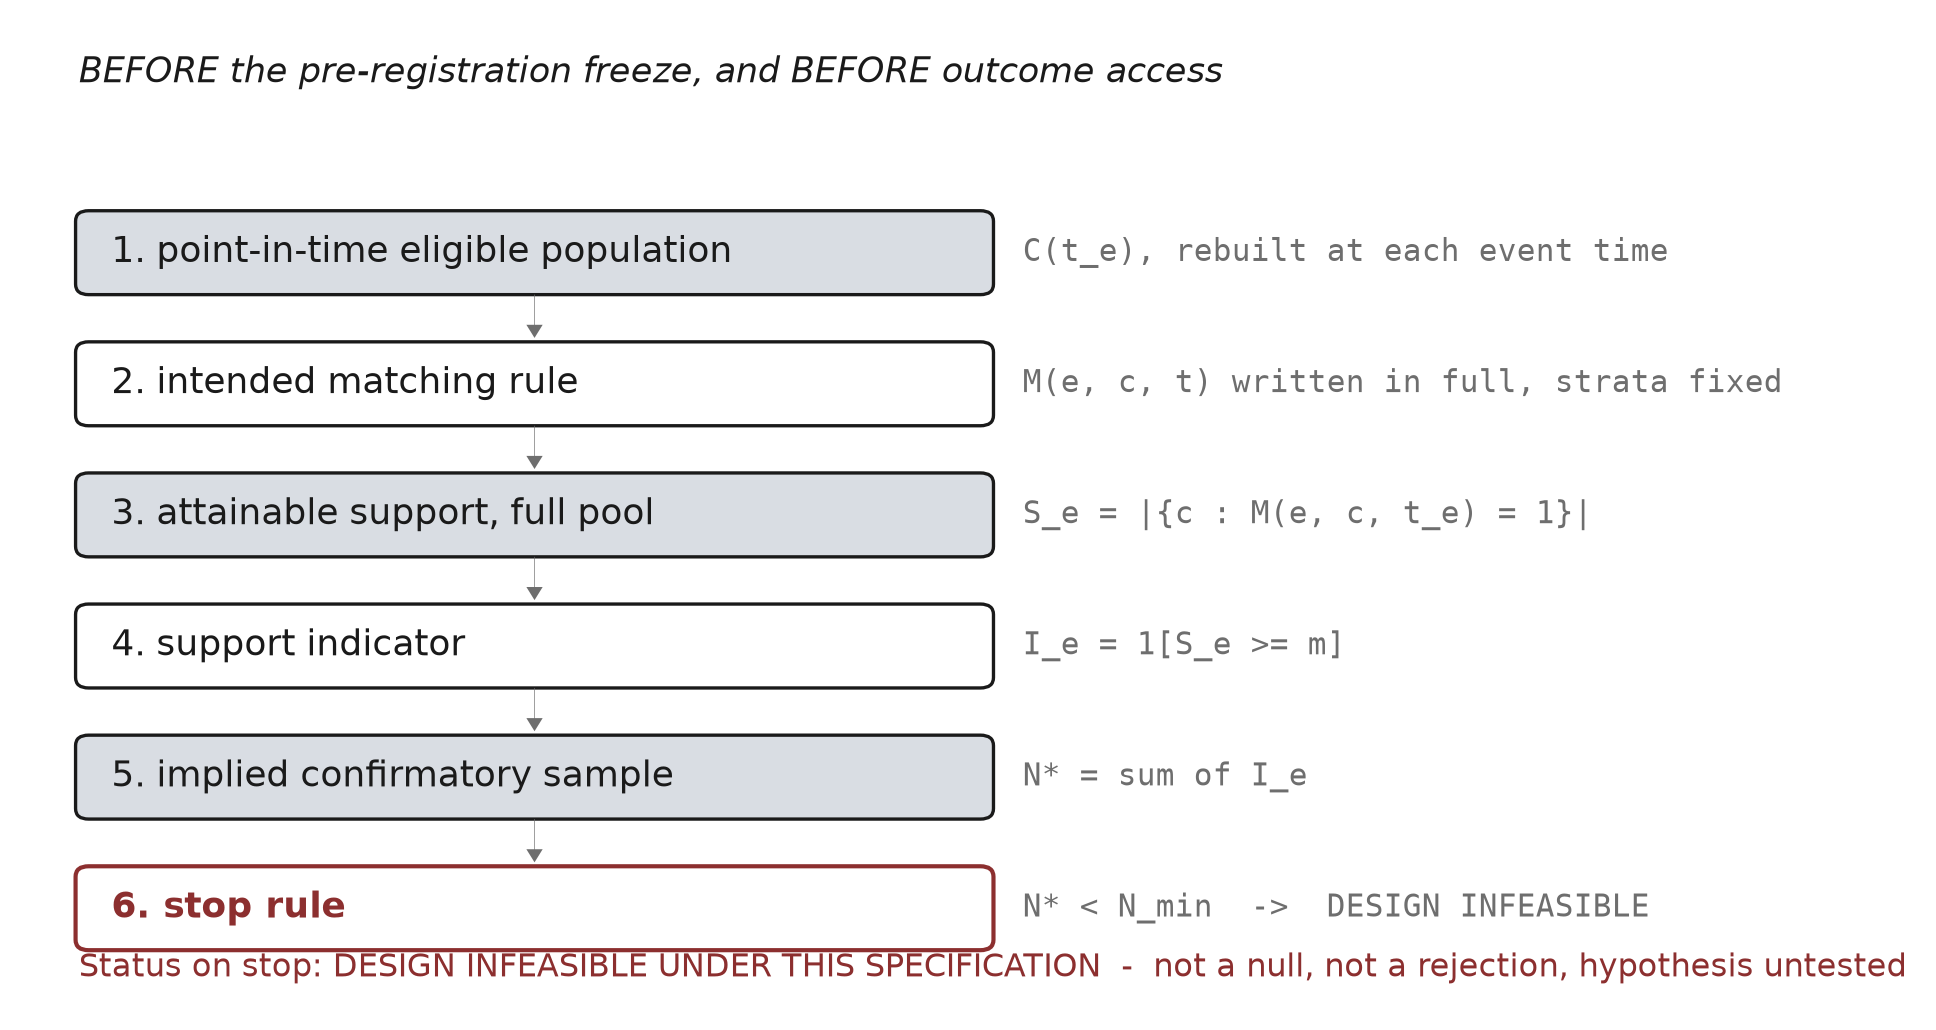
\includegraphics[width=\linewidth]{figures/v3_f1_procedure.png}
\end{center}


\textbf{Figure 1. The pre-freeze common-support audit.} Schematic of the procedure in \S{}2.3: the point-in-time eligible population at each event time, the intended matching rule, the attainable support \texttt{S\_e}, the support indicator, and the stop rule on \texttt{N*}. The audit sits before the pre-registration freeze and before any outcome access. No quantities. \emph{Source: \S{}2.3.}


\begin{center}
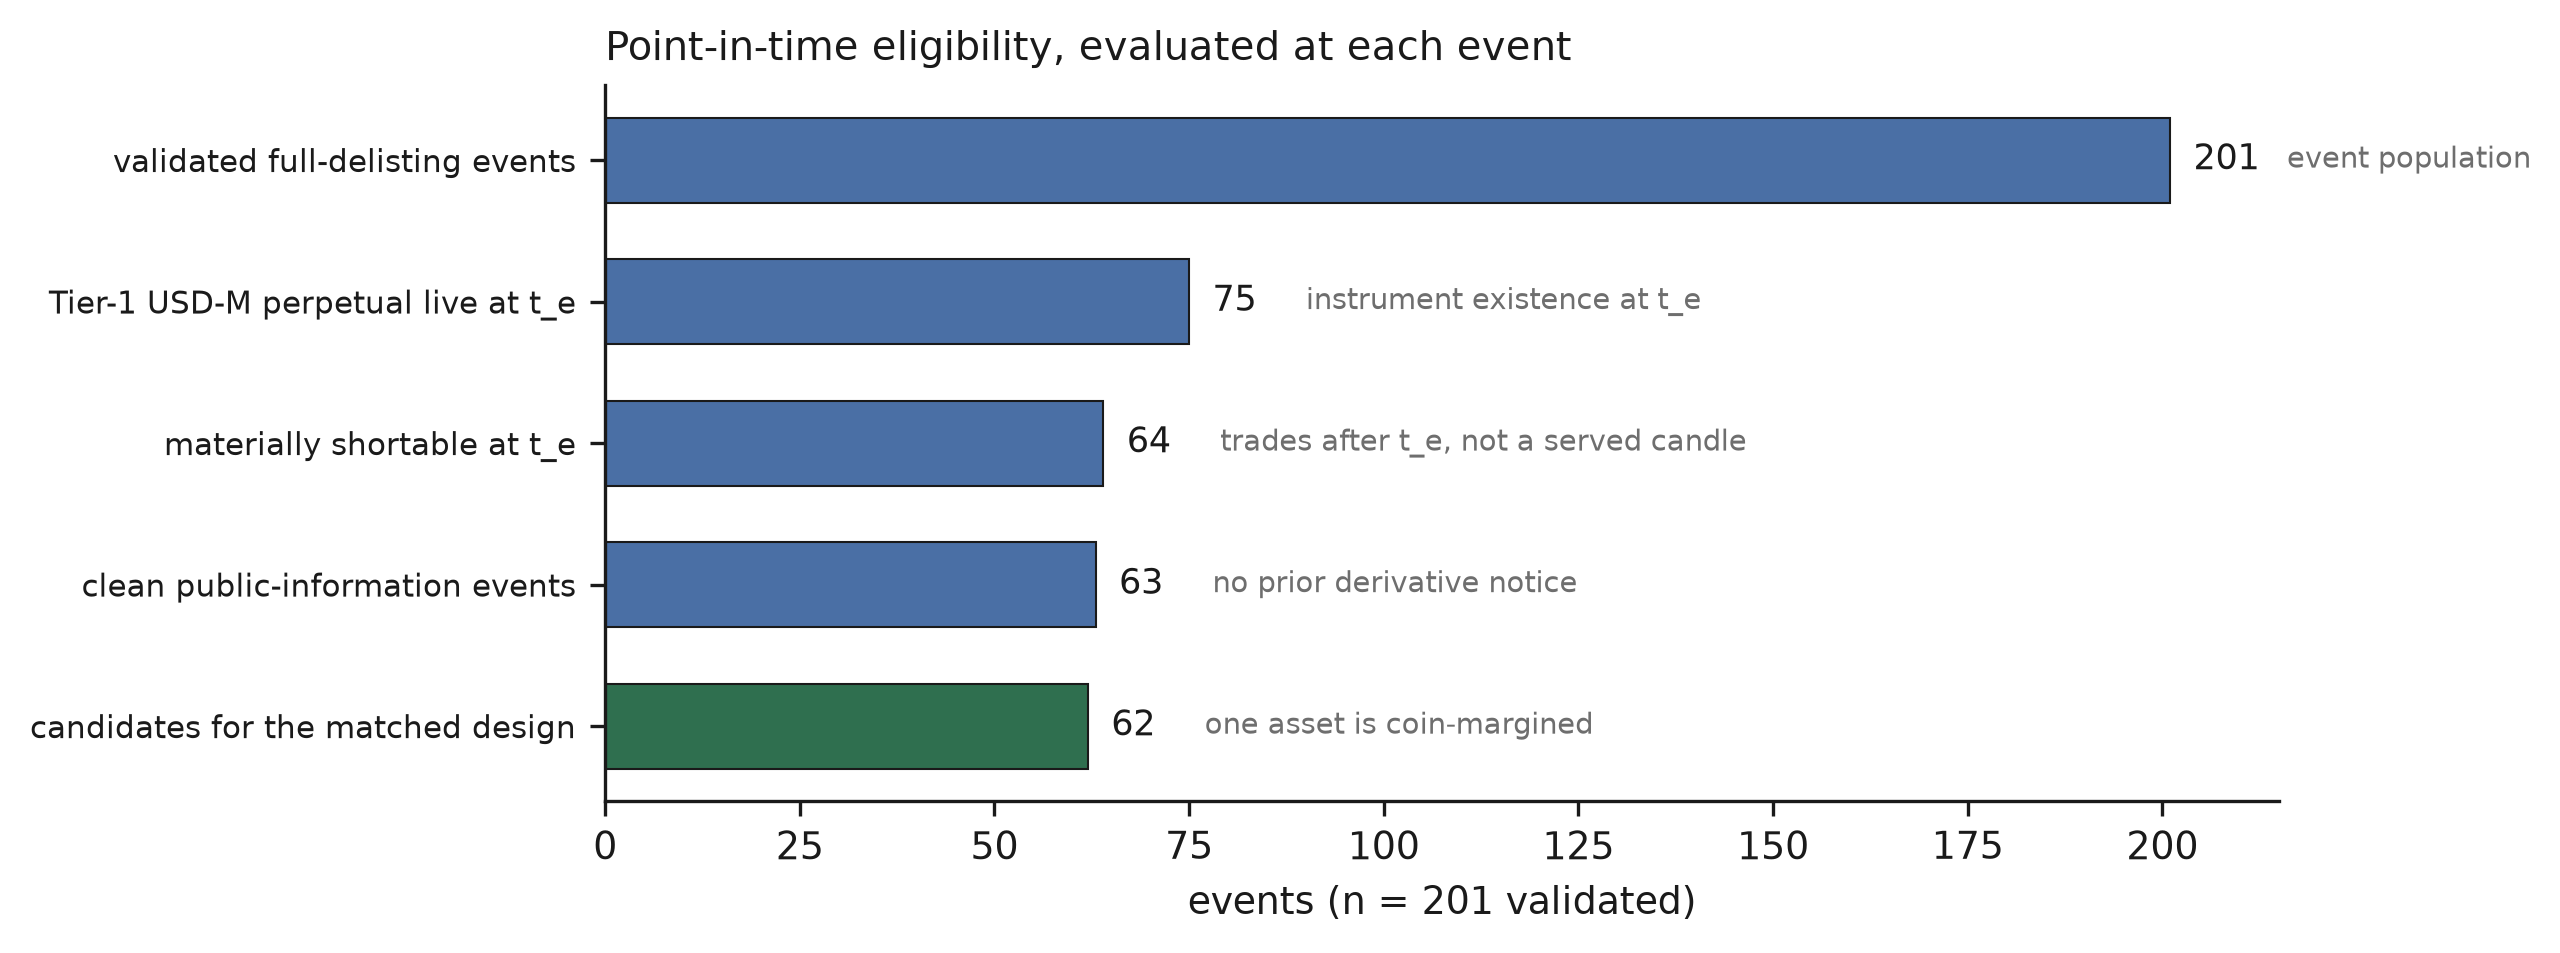
\includegraphics[width=\linewidth]{figures/v3_f2_event_funnel.png}
\end{center}


\textbf{Figure 2. From validated event population to candidate design.} Events, from n = 201 validated full-delisting events to the 62 that enter the matched design. Descriptive. Each reduction is a point-in-time eligibility condition evaluated at the event, not a filter applied with hindsight (\S{}4.1). \emph{Source: \texttt{H19\_0\_GATE.json}. Data: \texttt{figures/data/v3\_f2\_event\_funnel.csv}.}


\begin{center}
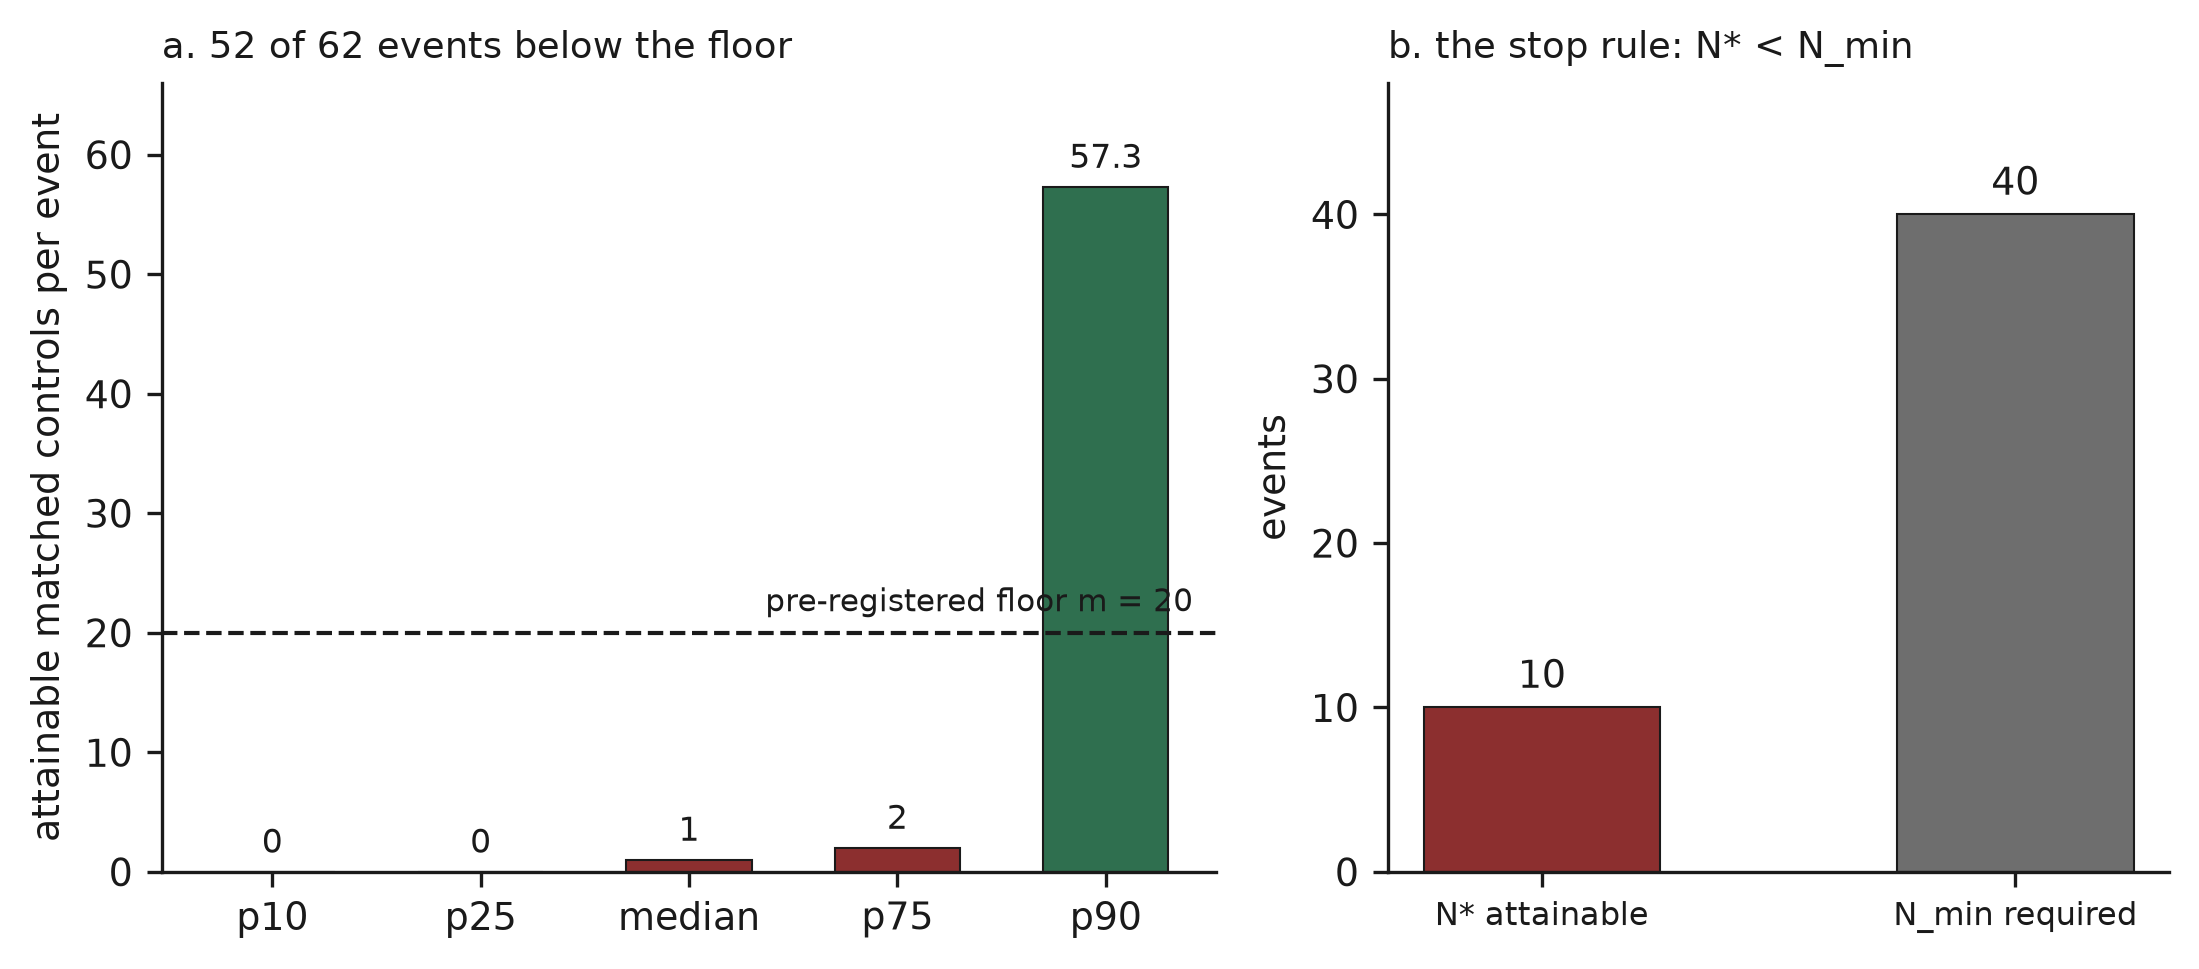
\includegraphics[width=\linewidth]{figures/v3_f3_support_audit.png}
\end{center}


\textbf{Figure 3. The central result: attainable matched support against the pre-registered floor.} Matched controls available per event, in controls, over n = 62 candidate events, with the frozen floor of 20 and the implied confirmatory sample N\textbackslash{}\emph{ = 10 against a required N\_min = 40. Descriptive, and outcome-blind: no price column was loaded at any point. 52 of 62 events fall below the floor; the distribution is bimodal because 52 of the 62 event assets carried the public warning (\S{}4.3). }Source: \texttt{data/alpha\_sprint/h19\_2\_prefreeze.json}. Data: \texttt{figures/data/v3\_f3\_support\_audit.csv}.*


\begin{center}
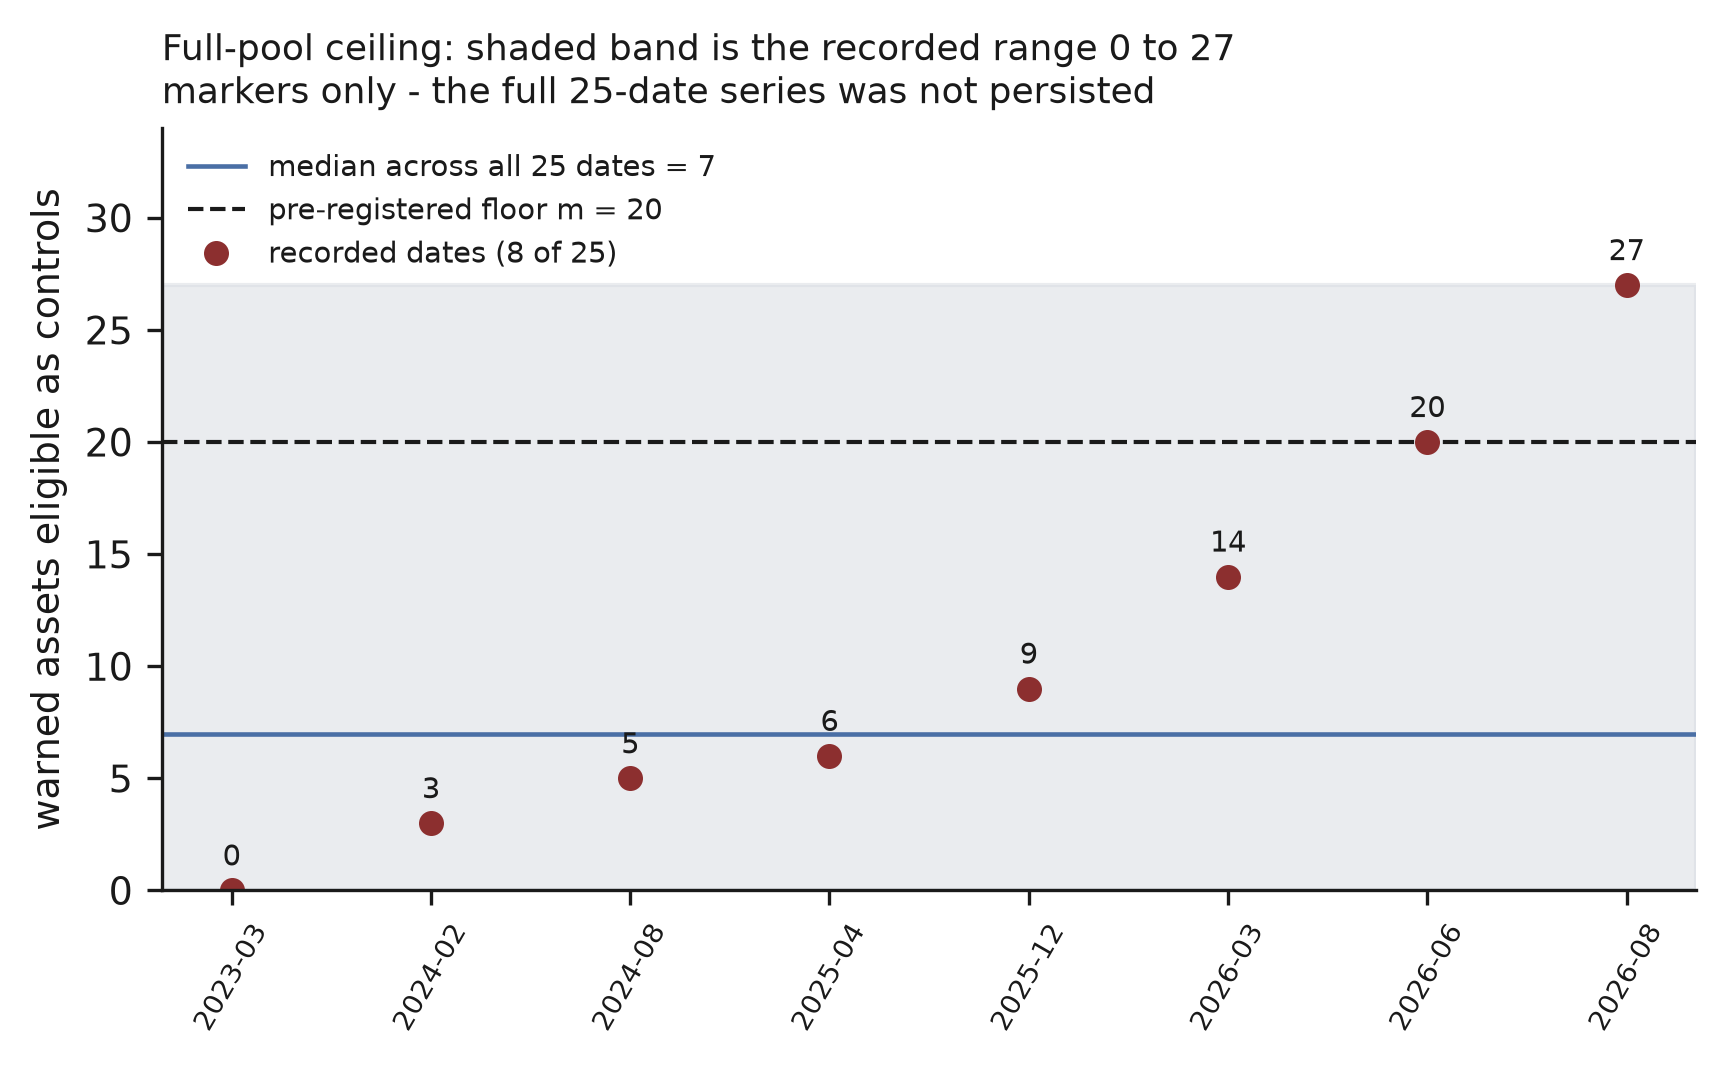
\includegraphics[width=\linewidth]{figures/v3_f4_full_pool_ceiling.png}
\end{center}


\textbf{Figure 4. The full-pool ceiling.} Warned assets simultaneously eligible as controls, in assets, at each announcement date, computed on the complete eligible pool with no sampling. Markers, not a connected series: the artefact records 8 of the 25 announcement dates, and the remaining 17 were summarised to a median rather than persisted, so the gaps are a limit of the record and are not interpolated. The band shows the recorded range (0 to 27) and the median across all 25 dates (7). Only 3 of 25 dates reach the floor of 20, before the liquidity band is matched (\S{}4.3). \emph{Source: \texttt{H19\_2\_PREFREEZE\_FEASIBILITY.md} Check 3. Data: \texttt{figures/data/v3\_f4\_full\_pool\_ceiling.csv}.}


\section*{Tables}


\begin{center}
\footnotesize
\begin{tabular}{p{0.307\linewidth}p{0.307\linewidth}p{0.307\linewidth}}
\hline
\textbf{\#} & \textbf{table} & \textbf{file} \\
\hline
T1 & the pre-freeze audit: inputs, computation and stop rule & \texttt{tables/v3\_table1\_procedure.md} \\
T2 & the H19.2 support audit, with every quantity and its artefact & \texttt{tables/v3\_table2\_support\_audit.md} \\
T3 & bounded supporting results & \texttt{tables/v3\_table3\_supporting.md} \\
\hline
\end{tabular}
\end{center}


Appendix tables: the full 31-entry registry (Appendix B), the threshold inventory (Appendix C), the failure taxonomy and implementation defects (Appendix D), and the full principle list (Appendix E).



\section*{Appendix A --- Supporting measurements and their artefacts}


\subsection*{A.1 Liquidity, reported as a distribution}


A liquidity screen was applied to the 63 clean information events in a separate feasibility gate, requiring that a US\$1,000 order be at most a stated fraction of median hourly notional. \textbf{The distribution is the result; the 1\% operating point is an engineering judgement.}


\begin{center}
\footnotesize
\begin{tabular}{p{0.307\linewidth}p{0.307\linewidth}p{0.307\linewidth}}
\hline
\textbf{order size as a share of median hourly notional} & \textbf{share of the 63 clean events} & \textbf{events} \\
\hline
$\leq$ 0.10\% & 3.17\% & 2 \\
$\leq$ 0.50\% & 33.33\% & 21 \\
$\leq$ 1.00\% & 50.79\% & \textbf{32} \\
\hline
\end{tabular}
\end{center}


The 32 figure is one labelled operating point on this distribution and is reported as such. The underlying liquidity of the clean sample: 31 events trade below US\$100k per hour, 30 between US\$100k and US\$1m, and 2 above US\$1m.


\textbf{This is a screen, not an execution analysis.} It establishes instrument availability and coarse liquidity. It does not establish execution feasibility and is not a profitability result: no order book, spread, market impact, taker or maker fee, funding cost, latency, intraday volume distribution or fill-probability estimate was available or measured, and no return, carry or P\&L was computed for any event. For a sample in which half the events trade below US\$100k per hour, the spread alone could dominate any effect.


Margin-based shortability is \texttt{UNKNOWN}, not zero: no official keyless surface exposes historical margin eligibility, and inferring it from current support is forbidden by the same rule that forbids current instrument lists as history. The funnel in \S{}4.1 is therefore a lower bound.


\subsection*{A.2 Derivative notice coverage}


Across the 201 events, 12 carry a derivative notice after the spot announcement, 5 before it, and for \textbf{184 no derivative notice was found}. That is a limit of the official surfaces reached, \textbf{not 184 events proven to have had none}, and the announcement-ordering subgroup is declared not estimable rather than null.


\section*{Appendix B --- The full research registry}


Thirty-one entries across ten cycles. "Economic outcome computed" means an aggregate return, edge or P\&L figure was produced. Source: \texttt{docs/alpha\_sprint/HYPOTHESIS\_LEDGER.md}, the per-family gate artefacts, and the git history.


\begin{center}
\footnotesize
\begin{tabular}{p{0.115\linewidth}p{0.115\linewidth}p{0.115\linewidth}p{0.115\linewidth}p{0.115\linewidth}p{0.115\linewidth}p{0.115\linewidth}p{0.115\linewidth}}
\hline
\textbf{\#} & \textbf{family} & \textbf{stage reached} & \textbf{terminal state} & \textbf{econ. outcome} & \textbf{pre-registered} & \textbf{holdout} & \textbf{reference} \\
\hline
H1 & perp/quarterly regime switching & full test & \texttt{REJECT} & \textbf{yes} & yes & yes & \texttt{PREREGISTRATION.md} \\
H2 & funding settlement timing & partial test & \texttt{WATCH} & \textbf{yes} & yes & --- & \texttt{94052bf} \\
H3 & liquidation reversal & audit & \texttt{WATCH} $\rightarrow$ H3.1 & no & yes & --- & \texttt{PREREGISTRATION.md} \\
H3.1 & cascade exhaustion vs continuation & full test & \texttt{REJECT} & \textbf{yes} & yes & yes & \texttt{18c3f65} \\
H4 & cross-sectional funding/basis/momentum & full test & \texttt{REJECT} / \texttt{WATCH} & \textbf{yes} & yes & yes & \texttt{PREREGISTRATION.md} \\
H5.1 & CEX↔DEX funding fragmentation & full test & \texttt{REJECT} & \textbf{yes} & yes & yes & \texttt{fb9e6d1} \\
H6.1 & options volatility risk premium & full test & \texttt{REJECT} & \textbf{yes} & yes & yes & \texttt{16cc502} \\
H7.1 & prediction-market logical arbitrage & full test & \texttt{REJECT} & \textbf{yes} & yes & yes & \texttt{a8639ae} \\
H8.1 & cross-asset medium-horizon trend & full test & \textbf{\texttt{PROMOTED}} $\rightarrow$ paper portfolio & \textbf{yes} & yes & yes & \texttt{e771727}, \texttt{0e865bd} \\
H8.2 & allocation / overlay falsifications & falsification & \texttt{KEEP H8.1} & \textbf{yes} & yes & --- & \texttt{032fc25} \\
H9 & prediction-market favourite premium & full test & \texttt{REJECT} & \textbf{yes} & yes & yes & \texttt{756719f} \\
H10 & odd-lot priority in tender offers & full test & \texttt{REJECT} & \textbf{yes} & yes & yes & \texttt{5a7c7c1} \\
H11 & post-spin forced selling & full test & \texttt{REJECT} & \textbf{yes} & yes & yes & \texttt{6e5903f} \\
H12 & public-company liquidation discount & data phase & \texttt{RESEARCH (data)} & partial & yes & --- & \texttt{e2d5f71} \\
H13 & net-nets / cash shells & full test & \texttt{IMPLEMENTATION REJECT / ECONOMIC QUESTION UNRESOLVED} & \textbf{yes} & yes & yes & \texttt{aca53bf} \\
H14 & B3 deep special situations & universe only & \textbf{\texttt{OPEN}} & no & no & --- & \texttt{61f0bc8} \\
H14.1 & B3 takeover-offer terms & gate & \texttt{DATA-GATE FAIL} & no & no & --- & \texttt{7c44e67} \\
H14.2 & B3 judicial reorganisation & gate (1 of 7) & \texttt{DATA-GATE FAIL} & no & no & --- & \texttt{58bd03f} \\
H14.3 & B3 recapitalisations and rights & gate (0 of 9) & \texttt{DATA-GATE FAIL} & no & no & --- & \texttt{eabd336} \\
H15 & Schedule 13D activist & gate (5 of 22) & \texttt{DATA-GATE FAIL / UNTESTED} & no & no & --- & \texttt{cb722dd} \\
H16.1 & FDA / PDUFA binary catalysts & gate (2 of 23) & \texttt{DATA-GATE FAIL / UNTESTED} & no & no & --- & \texttt{dcefafe} \\
H17.0 & historical market data for Form 4 & gate (14 of 32) & \texttt{INFRASTRUCTURE BLOCKED} & no & no & --- & \texttt{e96ba10} \\
H18.0 & three-venue delisted-OHLCV probe & gate & \texttt{INFRASTRUCTURE BLOCKED} & no & no & --- & \texttt{6f7dbf4} \\
H18.0b & venue substrate confirmation & gate (14 of 14) & \texttt{PASS} (substrate) & no & no & --- & \texttt{55f68ec} \\
H18.1 & spot lifecycle semantic audit & gate (11 of 12) & \texttt{PARTIAL PASS} & no & no & --- & \texttt{2a746cc} \\
H18.1b & full-delisting universe expansion & gate (19 of 19) & \texttt{STRONG PASS} & no & no & --- & \texttt{27c3283} \\
H18.2 & hypothesis selection & selection & \texttt{SELECT} & no & n/a & --- & \texttt{45d575d} \\
H18.3 & route contraction $\rightarrow$ 365-day risk & full pre-registered test & \textbf{\texttt{PRE-REGISTERED NULL}} & no (PR-AUC only) & \textbf{yes, hashed} & \textbf{yes, once} & \texttt{522bafb}, \texttt{203390b}, \texttt{4aa4180} \\
H19.0 & execution / shortability gate & gate (12 of 15) & \texttt{PARTIAL PASS} / capacity screen & no & no & --- & \texttt{320ce41} \\
H19.1 & derivative price-discovery selection & selection & \texttt{SELECT} + 3 modifications & no & n/a & --- & \texttt{564baf8} \\
H19.2 & derivative-specific pre-delisting discovery & \textbf{pre-freeze feasibility} & \textbf{\texttt{DESIGN INFEASIBLE UNDER THIS SPECIFICATION}} & \textbf{no --- no price read} & \textbf{no --- never frozen} & no & \texttt{42f35df} \\
\hline
\end{tabular}
\end{center}


\section*{Appendix C --- Threshold inventory}


Nineteen decision thresholds, classified. None is \texttt{THEORETICAL}; two are \texttt{CONVENTIONAL}; the remainder are \texttt{ENGINEERING JUDGEMENT}. Three conclusions in the wider program are threshold-determined: the infeasibility verdict in \S{}4.4 follows from \emph{m} = 20; the 32 operating point in Appendix A.1 follows from the 1\% rule; and a materiality criterion in \S{}6.3 follows from a calibration bar that is defective as written, penalising improvement as well as deterioration.


\textbf{Pre-specification protects against outcome-driven threshold movement; it does not make an arbitrary threshold theoretically correct.} Bars fall into four levels: derived from a model (none here); borrowed from an established convention (two); engineering judgement fixed before measurement and not moved (the rest); and chosen after seeing the result (none, by construction). Level-3 discipline protects the sequence, not the value.


Full inventory: \texttt{tables/v3\_appendix\_thresholds.md}.


\section*{Appendix D --- Failure taxonomy and implementation defects}


Classes of silent failure that produced plausible output --- source coverage and truncation, format-change false horizons, unit-convention divergence between two legs of one comparison, gate-metric truthiness recurring across two families, and classification-level future information --- are in \texttt{tables/v3\_appendix\_failure\_taxonomy.md}. Local implementation defects, retained for completeness and \textbf{not claimed as contributions}, are in \texttt{tables/v3\_appendix\_defects.md}. Discovering one's own defect carries no information about markets.


\section*{Appendix E --- Principles}


Four principles are carried in the body of this paper:


\textbf{P1.} Point-in-time identity and eligibility must be constructed, not assumed. \textbf{P2.} A documented event is not automatically an executable or identifiable event. \textbf{P3.} Common-support feasibility can be measured on the full pool before outcome access. \textbf{P4.} Failure at a pre-outcome design gate is \texttt{NO\_TEST}, not an economic null.


The remaining six from earlier versions are in \texttt{tables/v3\_appendix\_principles.md}.



\section*{Data and code availability}


Every number maps to a row of \texttt{CLAIM\_EVIDENCE\_MATRIX\_V3.csv}. Artefacts, commits and hashes are indexed in \texttt{../ARTIFACT\_INDEX.md}; environment, seeds and state transitions in \texttt{../REPRODUCIBILITY\_APPENDIX.md}. Figures and tables regenerate from committed artefacts via \texttt{scripts/paper\_build\_v3.py}; audits run via \texttt{scripts/paper\_audit\_v3.py}. \textbf{No public repository or DOI exists yet}, and the manuscript has never been compiled: no LaTeX distribution is available in the environment used.


\section*{Evidence classes}


Four categories, never blended within a claim: \textbf{internal empirical evidence} (this program's experiments), \textbf{external literature} (with access level stated per entry), \textbf{official venue documentation}, and \textbf{paid reference} (none used).


\section*{References}


See \texttt{references\_v3.bib}.


\end{document}
